\chapter{Operations}



%Numbers come in a lot of different forms. We all know that 2 is a number. Many of us have seen $\pi$ in some capacity and recognize that it is a number. In a similar manner, you may know that $\sqrt{9001}$ and $3i + 17$ are numbers. But without understanding what these numbers mean, they are worthless. The first step in our journey towards establishing meaning for numbers starts with classification of these numbers.

%\begin{presentation}
%\begin{defn}[Number Set]\label{defn1}
%	A number set is a collection of numbers.
%\end{defn}
%\end{presentation} \index{Number Set}

%First definition down. This is a small, but significant definition as well. Number sets will be a recurring character throughout this book. 

%\begin{defn}[Natural Number]\label{defn2}
%	A number is called natural if we can use it to count. We denote the set of natural numbers as $\mathbb{N}$. \\ $1,2,3,4,$ and $5$ are examples natural numbers.
%\end{defn}

%We use natural numbers every single day. However, there are some quantities that we cannot describe using natural numbers. Enter the integers.

%\begin{presentation}
%\begin{defn}[Integer]
%	A number is an integer if it has no fractional part. An integer can be either positive or negative. We denote the set of integers as $\mathbb{Z}$. \\$-4, -2, 0, 3,17,  9002$ are all examples of integers. 
%\end{defn}
%\end{presentation}

%We can use number lines to plot integers.

%\vspace{2cm}

%\numline









 %Integers are also where we introduce mathematical operations. 

Our goal this semester is to have a strong understanding of both linear and quadratic functions. Before we dive in, let's review some of the tools we are going to use all semester. 
\begin{presentation}
\begin{defn}[Variable]
	A variable is a representation for an unknown quantity. We traditionally use letters as variables. 
\end{defn}
\end{presentation}

Outside of math, the word variable is defined as ``apt or liable to vary or change''.\footnote{\texttt{www.dictionary.com}} Within math it really means the same thing. We use variables for unknown quantities or changing quantities because it makes understanding functions way easier. These are going to be our most frequently used tool this semester. 

\begin{center}
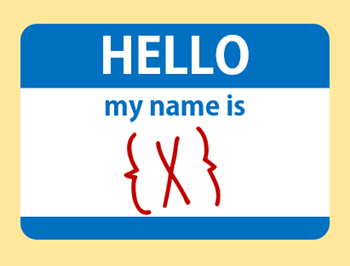
\includegraphics[scale=.75]{variable.png}
\end{center}

\begin{defn}[Elementary Operation]
An operation is a calculation that is done using some combination of numbers. The four elementary operations are addition (+), subtraction (-), multiplication ( $\cdot$ or $\times$), and division ($\div$ or $/$ ).
\end{defn}

%The addition of two numbers is the combination of the two quantities. We can represent this operation on a number line.
%\begin{example}[Addition on a Number Line]
%	To visualize addition on a number line, start by plotting the first number on the number line. Consider $3+-6$.
%	
%	\begin{center}
%	\begin{tikzpicture}
%	\draw[latex-] (-6.5,0) -- (6.5,0) ;
%	\draw[-latex] (-6.5,0) -- (6.5,0) ;
%	\foreach \x in  {-5,-4,-3,-2,-1,0,1,2,3,4,5}
%	\draw[shift={(\x,0)},color=black] (0pt,3pt) -- (0pt,-3pt);
%	\foreach \x in {-5,-4,-3,-2,-1,0,1,2,3,4,5 }
%	\draw[shift={(\x,0)},color=black] (0pt,0pt) -- (0pt,-3pt) node[below] 
%	{$\x$};
%	\end{tikzpicture}
%	\end{center}


%	\begin{center}
%	\begin{tikzpicture}
%\begin{axis}[
%  axis y line=none,
%  axis lines=left,
%  axis line style={-},
%  xmin=-11,
%  xmax=11,
%  ymin=0,
%  ymax=1,
%  scatter/classes={o={mark=*}},
%  restrict y to domain=0:1,
%  xtick={-10,-9,-8, ...,10},
%  width=16cm
%]
%\addplot table [y expr=0,meta index=1, header=false] {
%114.06 o
%119.94 o
%};
%\node[coordinate,label=above:{$L_1=114.06$}] at (axis cs:114.06,0.05) {};
%\node[coordinate,label=above:{$L_2=119.94$}] at (axis cs:119.94,0.05) {};
%\end{axis}
%\end{tikzpicture}
%	\end{center}

%\end{example}

However, these are not the only operations we are going to use during this class. 

\begin{defn}[Exponent]
An exponent is a representation of the power of an expression. When dealing with positive exponents, this is a fancy way of saying the exponent is the number of times you multiply an expression by itself. The following table shows how to do this for a number $n$:
$$
\begin{array}{|ccl|}
\hline 
n^3 & = & 1 \cdot (n \cdot n \cdot n) \\
n^2 & = & 1 \cdot (n \cdot n) \\
n^1 & = & 1 \cdot( n )\\
n^0 & = & 1 \\
n^{-1} & = & 1 \div (n) \\
n^{-2} & = & 1 \div (n \cdot n) \\
n^{-3} & = & 1 \div (n \cdot n \cdot n)\\
\hline
\end{array}
$$ 
\end{defn}






\begin{defn}[Fraction]
	A fraction is a number that expresses some part of an integer. It can also be viewed as an integer divided by an integer. 
\end{defn}

The reason why a definition for a fraction is included here is because fractions tend to confuse many students. However, a fraction is simply a number dividing another number. If we try to only think of fractions as this, hopefully our confusion will be minimized. 
